\begin{frame}
\titlepage
\end{frame}


\section{Intro}

\begin{frame}{Roadmap}
    \begin{itemize}
        \item The challenge of nonlocal phonotactics
        \item SP phonotactic model
        \item Unsupervised Learning
        \item Case study: Quechua
    \end{itemize}
\end{frame}

% \section{Nonlocal phonotactics}

\begin{frame}{Phonotactics}
\begin{itemize}
\item The speakers' knowledge of possible and impossible sound sequences:\\
\begin{center}
\begin{tabular}{cll}
\textit{\textbf{br}ick}& Existing  & well-formed\\
\textit{\textbf{bl}ick}&Nonexisting  &  well-formed\\
*\textit{\textbf{bn}ick}&Nonexisting  & ill-formed
\end{tabular}
\end{center}
\hfill \small \citep{chomsky1965some,hayes2008maximum}

\item Phonotactic learning is a crucial aspect of phonological acquisition and has figured significantly in computational phonology.
\hfill \small \citep{}
\end{itemize}

\end{frame}

\begin{frame}{Baseline: {local} $n$-grams}

\begin{itemize}
    \item $n$-gram: contiguous sequence of $n$ items;
%\hfill \small\citep{markov1913essai}
    \item Imagine a learner only observed one word $abcd$:\\
    \begin{center}
    \begin{tabular}{lcc}
        $n$ & legal local $n$-grams & illegal local $n$-grams\\\midrule
        $1$ & $a$, $b$, $c$, $d$ & *$e$, *$f$, *$\smiley$ \ldots\\
        $2$ & $ab$, $bc$, $cd$ & *$aa$, *$ac$, *$ad$ \ldots\\
        $3$ & $abc$, $bcd$ & *$aaa$, *$bbb$\ldots \\
        % $4$ & $abcd$
    \end{tabular}
    \end{center}
    % \item Unigrams: the alphabet $\{a,b,c,d\}$.
  \onslide<2-> {\item Previous works usually hypothesize \textbf{local} $n$-grams as the free parameters/constraints (grammar) of the phonotactic learner \citep{hayes2008maximum}.
  

    \item E.g.\ *$aaaaa$ will not be accepted by the bi-/trigram constraints (*$aa$, *$aaa$). }
\end{itemize}


    
\end{frame}

\begin{frame}{Challenge: nonlocal phonotactics}
\begin{itemize}
\item The speakers' knowledge of possible and impossible \textbf{nonadjacent} sound sequences at \textbf{arbitrary} distance.
\item Sometime motivates long-distance di-/assimilation $\rightarrow$ harmony systems
%  \item The parameter space will explode if the learner memorizes local $n$-grams to approximate nonlocal phonotactics.
 
%  \item E.g.\ *tʃ\super h\ldots s/*s\ldots tʃ\super h in Ineseño Chumash.
 % learning a grammar is impossible since every time you create a new words, the learner has to memorize a some new ngrams.
 % this is computational intractable. 
 \end{itemize}
\end{frame}

\begin{frame}{Ineseño Chumash nonlocal sibilant phonotactics}
    
\begin{itemize}
\item In Ineseño Chumash, the co-occurrence of alveolar \{s, z, t͡s, d͡z,\ldots\} and lamino-postalveolar \{ʃ, ʒ, t͡ʃ, d͡, ʒ,\ldots\} sibilants is illegal e.g.\ $^{\ast}$ʃ\ldots s,  $^{\ast}$s\ldots ʃ.\vspace{-0.2cm}
\begin{columns}
\begin{column}{0.55\textwidth}
\begin{exe}
    \ex {ʃapitʃ\super holit} \hspace{0.5cm} /\textbf{s}-api-\textbf{tʃ\super h}o-it/ \par  `I have a stroke of good luck' 
    \ex {ʃapitʃ\super holuʃwaʃ} \hspace{0.5cm}  /ʃ-api-\textbf{tʃ\super h}o-u\textbf{s}-waʃ/  \par `He had a stroke of good luck'
    % \ex {sapits\super holus} /s-api-tʃ\super ho-us/ \hfill`He has a stroke of good luck'
    \ex *{sapitʃ\super holit}, *{ʃapitʃ\super holuswaʃ}
\end{exe}
\end{column}
\begin{column}{0.35\textwidth}
\vspace{0.5cm}
\begin{table}[]
    \centering
 \begin{tabular}{cc}%\toprule
     & 5-grams \\ \midrule
     & ʃapitʃ\super h\\
     & apitʃ\super ho \\
     & pitʃ\super hol\\
    %  & itʃ\super holi \\
     & \ldots   %\\\bottomrule
\end{tabular}
\end{table}
\hfill\small \citep{applegate1972ineseno}
\end{column}

\end{columns}

\end{itemize}

\end{frame}

\begin{frame}{Challenge: nonlocal phonotactics}
\begin{itemize}
\item The speakers' knowledge of possible and impossible nonadjacent sound sequences at \textbf{arbitrary} distance;

 \item The parameter space will explode if the learner memorizes local $n$-grams to approximate nonlocal phonotactics;
  \\
 \hfill\small\citep{hayes2008maximum,gouskova2019inducing}
\item Any such approximation also completely misses the generalization. 
 \\
 \hfill\small\citep{heinz2010maximum}
%  \item E.g.\ *tʃ\super h\ldots s/*s\ldots tʃ\super h in Ineseño Chumash.
 % learning a grammar is impossible since every time you create a new words, the learner has to memorize a some new ngrams.
 % this is computational intractable. 
\end{itemize}
\end{frame}

\begin{frame}{Tiers}

\begin{center}
\begin{tikzpicture}
\node[swap] at (0,0) (0) {s};
\node at (1,0) (1) {a};
\node at (2,0) (2) {p};
\node at (3,0) (3) {i};
\node at (4,0) (4) {tʃ\super h};
\node at (5,0) (5) {o};
\node at (6,0) (6) {l};
\node at (7,0) (7) {u};
\node at (8,0) (8) {s};
{\draw[solid, -] (0,0.75) node[above](t1){s} -- (0.north);
\draw[solid, -] (4,0.75) node[above](t2){tʃ\super h} -- (4.north);
\draw[solid, -] (8,0.75) node[above](t3){s} -- (8.north);}
\end{tikzpicture}  
\end{center}

\begin{itemize}
    \item Learning local $n$-gram on tiers/projections might work, while it also complicates the learning problem, e.g.\ learning tiers and multi-tier interactions.
    \hfill \small \citep{hayes2008maximum,gouskova2019inducing}
\normalsize
    \item Tier-based learner also predicts unattested \textit{blocking} effects.
    
    \hfill \small \citep{heinz2010learning,rose2004typology,hansson2010consonant}

\end{itemize}
\end{frame}

\begin{frame}{Goals and contributions}

    \begin{itemize}
        \item Modeling and learning nonlocal phonotactics \textbf{without tiers};
        \item Contra \citet{gouskova2019inducing}, it is possible to efficiently search through `nonlocal n-grams' by factored finite-state automata;  
        \item Integrating Formal Language Theory and statistical learning to handle noisy corpus data, and to predict the gradient acceptability of nonce forms.
    \end{itemize}
\end{frame}

\section{Strictly Piecewise phonotactic model}

% \begin{frame}{Subregular Hypothesis}

% Most phonological generalizations live in a \textbf{subregular} region in Chomsky Hierarchy which can be characterized by \textbf{restrictive} logical power and \textbf{deterministic} finite-state automata.\hfill\small\citep{heinz2018computational}

% \begin{figure}[H]
% % \vspace{-.3cm}
% \begin{center}
% \scalebox{0.78}{
%  \begin{tikzpicture}[
%     scale=5,
%     axis/.style={very thick, ->, >=stealth'},
%     important line/.style={thick},
%     dashed line/.style={dashed, thin},
%     pile/.style={thick, ->, >=stealth', shorten <=2pt, shorten
%     >=2pt},
%     every node/.style={color=black}
%     ]
%     % axis
%     \draw[axis] (0,0)  -- (1.1,0) node(xline)[right]
%         {$\begin{array}{l}\text{Relational}\\\text{structures}\end{array}$};
%     \draw[axis] (0,0) -- (0,1.1) node(yline)[above] {Logical power};
% \path[thick] (-0.5,0.23) edge[-,dashed] (1.1,0.23);
% \path[thick] (-0.5,0.45) edge[-,dashed] (1.1,0.45);
% \path[thick] (-0.5,0.78) edge[-,dashed] (1.1,0.78);
% \node(cnl) at (-0.3,0.1){$\begin{array}{c}\text{\small Conjunctions of}\\\text{\small Negative Literals}\end{array}$};
% \node(pp) at (-0.3,0.33){$\begin{array}{c}\text{\small Propositional}\end{array}$};
% \node(fo) at (-0.3,0.53){$\begin{array}{c}\text{\small First Order}\end{array}$};
% \node(mso) at (-0.3,0.9){$\begin{array}{c}\text{\small Monadic}\\ \text{\small Second Order}\end{array}$};
% \node(sl) at (0.25,-0.1){$+1$};
% \node(sp) at (0.7,-0.1){$<$};
% \node(sl) at (0.25,0.1){SL};
% \node[cadmiumred](sp) at (0.7,0.1){\textbf{SP}};
% \node(lt) at (0.25,0.33){LT};
% \node(pt) at (0.7,0.33){PT};
% \node(ltt) at (0.25,0.55){LTT};
% \node(sf) at (0.7,0.68){SF};
% \node(rg) at (0.45,0.9){Regular};
% \draw[-] (sl) -- (lt) -- (ltt) -- (rg);
% \draw[-] (ltt) -- (sf);
% \draw[-] (sp) -- (pt) -- (sf) -- (rg);
% \node[draw,align=left] at (2,0.7) {SL: Strictly Local\\ LT: Locally Testable\\ LTT: Locally-threshold Testable\\ SP: Strictly Piecewise\\ PT: Piecewise Testable\\ SF: Star Free};
% \end{tikzpicture}
%  }\vspace{-0.3cm}
% % \caption{Sub-regular Hierarchy } \label{fig:subregular}
% \end{center}
% \end{figure}

% % This computational characterization of phonological typology leads to the argument that, any computational modeling of phonological \textbf{learning} should search through this restrictive region instead of the intractable space to be faithful to human cognition. 
% % Moreover, all the Subregular languages can be characterized by {Deterministic} Finite-state Autotmata, which determines the shape of SP phonotactic model in the current study.
%     % \item I've shown how to integrate subregular approaches and statistical learning;

% \end{frame}


\begin{frame}{Nonlocal $n$-grams}
\begin{itemize}
\item Strictly Piecewise (SP) \textbf{grammar} evaluates \textbf{nonlocal} $n$-grams (subsequences).  e.g.\ given a legal string $abcd$:\\
\begin{center}
\begin{tabular}{ll}
        $n$ & legal nonlocal $n$-grams\\\midrule
        % $1$ & $a$, $b$, $c$, $d$  \\
        $2$ & $ab$, $ac$, $ad$, $bc$, $bd$, $cd$,  \\
        $3$ & $abc$, $abd$, $acd$, $bcd$ \\
        % $4$ & $abcd$
\end{tabular}
\end{center}

\item \textbf{SP languages}: Stringsets accepted by a SP grammar, e.g.\ \textit{abc}, \textit{abd} fir the bigrams here.
\item The number of nonlocal $n$-grams rapidly increase as a function of word length.
\end{itemize}

% \pagebreak

% \begin{quote}
%     Devising a computationally efficient search through nonlocal trigrams composed of natural class matrices will require a sophisticated implementation that \textbf{to the best of our knowledge is currently lacking}.
% \end{quote}
%How to efficiently evaluate them?
\vspace{-0.3cm}
\hfill\small \citep{gouskova2019inducing}
\end{frame}

\begin{frame}{Ineseño Chumash revisit}
        \begin{columns}
\begin{column}{0.55\textwidth}
\begin{exe}
    \ex {ʃapitʃ\super holit} \hspace{0.5cm} /\textbf{s}-api-\textbf{tʃ\super h}o-it/ \par  `I have a stroke of good luck' 
    \ex {ʃapitʃ\super holuʃwaʃ} \hspace{0.5cm}  /ʃ-api-\textbf{tʃ\super h}o-u\textbf{s}-waʃ/  \par `He had a stroke of good luck'
    % \ex {sapits\super holus} /s-api-tʃ\super ho-us/ \hfill`He has a stroke of good luck'
    \ex *{sapitʃ\super holit}, *{ʃapitʃ\super holuswaʃ}
\end{exe}
\end{column}
\begin{column}{0.35\textwidth}
\vspace{0.5cm}
\begin{table}[]
    \centering
 \begin{tabular}{cc}%\toprule
\multicolumn{2}{l}{nonlocal 2-grams} \\ \midrule
     ʃ\ldots tʃ\super h & {}^{*}s\ldots tʃ\super h\\
    %  &  \\
      tʃ\super h\ldots ʃ & {}^{*}tʃ\super h\ldots s\\
    %  & itʃ\super holi \\
      ʃ\ldots ʃ & {}^{*}s\ldots ʃ \\
      \ldots &\ldots \\\bottomrule
\end{tabular}
\end{table}
% \hfill\small \citep{applegate1972ineseno}
\end{column}
\end{columns}
\end{frame}

\begin{frame}{Solution: SP phonotactic model}
\begin{columns}
\begin{column}{0.55\textwidth}
\begin{itemize}
    \item A set of {Probabilistic Deterministic Finite-state Automata} (PDFAs) which characterizes Strictly Piecewise language.
    \item $\{\mathcal{M_{\text{1}}}, \mathcal{M_{\text{2}}}\}$ bans $\{{}^{\ast}\textcolor{bleudefrance}{a}\ldots\textcolor{cadmiumred}{a}, {}^{\ast}\textcolor{bleudefrance}{b}\ldots\textcolor{cadmiumred}{b}\}$ with the alphabet $A=\{a, b\}$. 
\end{itemize}
\end{column}
\begin{column}{0.45\textwidth}
\vspace{0.2cm}

\begin{tikzpicture}[shorten >=0.7pt, auto,thick,initial text=, minimum size=0pt]
\node[] at (1.5,-1) (q0) {\large \textbf{(a)} $\mathcal{M_{\text{1}}}$};
\node[state, initial, accepting,label={[label distance=0.2cm]270:{}}] (q1) {$a_0$};
\node[state, accepting,label={[label distance=0.2cm]270:{}}] at (3, 0) (q2) {$a_1$};
\draw  (q1) edge[loop above] node[text width=1.3cm]{$b: 0.5$} (q1)
(q2) edge[loop above] node[text width=1.3cm]{$a: 0 $ $b: 1 $} (q2);
\draw[->]  (q1) edge [above]  node  {$a: 0.5$}  (q2);
\end{tikzpicture}
\begin{tikzpicture}[shorten >=0.7pt, auto,thick,initial text=,minimum size=0pt]
 \node[] at (1.5,-1) (q0) {\large \textbf{(b)} $\mathcal{M_{\text{2}}}$};
\node[state, initial, accepting,label={[label distance=0.2cm]270:{}}] (q1) {$b_0$};
\node[state, accepting,label={[label distance=0.2cm]270:{}}] at (3, 0) (q2) {$b_1$};
\draw  (q1) edge[loop above] node[text width=1.3cm]{$a: 0.5$ } (q1)
(q2) edge[loop above] node[text width=1.3cm]{$a: 1$ $b: 0$} (q2);
\draw[->]  (q1) edge [above]  node  {$b: 0.5$}  (q2);
\end{tikzpicture}
\end{column}
\end{columns}
\end{frame}

\begin{frame}{Target symbol}
\begin{columns}
\begin{column}{0.55\textwidth}
\begin{itemize}
    \item Each factored automaton $\mathcal{M}$ only checks if it has seen one specific \textbf{target symbol} $\sigma$;
    \item No $\Rightarrow$ stay in state $\sigma_{0}$;
    \item Yes $\Rightarrow$ go to state $\sigma_{1}$;

    % \item The state $q$ of a symbol is decided by any preceding symbol.
    % \item The parameters are transition probabilities $T(\mathcal{M}, q, \sigma)$ given the segment $\sigma$ and state $q$ in $\mathcal{M}$.
\end{itemize}
\end{column}
\begin{column}{0.45\textwidth}
\vspace{0.2cm}

\begin{tikzpicture}[shorten >=0.7pt, auto,thick,initial text=, minimum size=0pt]
\node[] at (1.5,-1) (q0) {\large \textbf{(a)} $\mathcal{M_{\text{1}}}$};
\node[state, initial, accepting,label={[label distance=0.2cm]270:{}}] (q1) {$a_0$};
\node[state, accepting,label={[label distance=0.2cm]270:{}}] at (3, 0) (q2) {$a_1$};
\draw  (q1) edge[loop above] node[text width=1.3cm]{$b: 0.5$} (q1)
(q2) edge[loop above] node[text width=1.3cm]{$a: 0 $ $b: 1 $} (q2);
\draw[->]  (q1) edge [above]  node  {$\textcolor{cadmiumred}{a}: 0.5$}  (q2);
\end{tikzpicture}
\begin{tikzpicture}[shorten >=0.7pt, auto,thick,initial text=,minimum size=0pt]
 \node[] at (1.5,-1) (q0) {\large \textbf{(b)} $\mathcal{M_{\text{2}}}$};
\node[state, initial, accepting,label={[label distance=0.2cm]270:{}}] (q1) {$b_0$};
\node[state, accepting,label={[label distance=0.2cm]270:{}}] at (3, 0) (q2) {$b_1$};
\draw  (q1) edge[loop above] node[text width=1.3cm]{$\textcolor{cadmiumred}{a}: 0.5$ } (q1)
(q2) edge[loop above] node[text width=1.3cm]{$a: 1$ $b: 0$} (q2);
\draw[->]  (q1) edge [above]  node  {$b: 0.5$}  (q2);
\end{tikzpicture}
\end{column}
\end{columns}
\end{frame}


\begin{frame}{State}
\begin{columns}
\begin{column}{0.55\textwidth}
\begin{itemize}
    % \item Each factored automaton $\mathcal{M}$ only memorizes one \textbf{target symbol} on edge from $\sigma_0$ to $\sigma_1$.
    \item The state $q$ of a symbol is decided by any preceding symbol. 
    \item E.g.\ The second $a$ in *$aa$ is in $a_1$ in $\mathcal{M_{\text{1}}}$, and $b_0$ in $\mathcal{M_{\text{2}}}$.  
\end{itemize}
\end{column}
\begin{column}{0.45\textwidth}
\vspace{0.2cm}

\begin{tikzpicture}[shorten >=0.7pt, auto,thick,initial text=, minimum size=0pt]
\node[] at (1.5,-1) (q0) {\large \textbf{(a)} $\mathcal{M_{\text{1}}}$};
\node[state, initial, accepting,label={[label distance=0.2cm]270:{}}] (q1) {$a_0$};
\node[state, accepting,label={[label distance=0.2cm]270:{}}, fill=gray!30] at (3, 0) (q2) {$a_1$};
\draw  (q1) edge[loop above] node[text width=1.3cm]{$b: 0.5$} (q1)
(q2) edge[loop above] node[text width=1.3cm]{$a: 0 $ $b: 1 $} (q2);
\draw[->]  (q1) edge [above,cadmiumred]  node  {$a: 0.5$}  (q2);
\end{tikzpicture}
\begin{tikzpicture}[shorten >=0.7pt, auto,thick,initial text=,minimum size=0pt]
 \node[] at (1.5,-1) (q0) {\large \textbf{(b)} $\mathcal{M_{\text{2}}}$};
\node[state, initial, accepting,label={[label distance=0.2cm]270:{}}, fill=gray!30] (q1) {$b_0$};
\node[state, accepting,label={[label distance=0.2cm]270:{}}] at (3, 0) (q2) {$b_1$};
\draw  (q1) edge[loop above,cadmiumred] node[text width=1.3cm]{$a: 0.5$ } (q1)
(q2) edge[loop above] node[text width=1.3cm]{$a: 1$ $b: 0$} (q2);
\draw[->]  (q1) edge [above]  node  {$b: 0.5$}  (q2);
\end{tikzpicture}
\end{column}
\end{columns}
\end{frame}


\begin{frame}{Parameters}
\begin{columns}
\begin{column}{0.55\textwidth}
\begin{itemize}
    \item The parameters are transition probabilities $T(\mathcal{M}, q, \sigma)$ conditioned by the segment $\sigma$ and state $q$ in $\mathcal{M}$.
    \item \textbf{Interpretable} as the probabilities of subsequences.
    \item E.g.\  $\textsf{Pr}([a\ldots a])<\textsf{Pr}([a\ldots b])$, $\textsf{Pr}([b\ldots b])<\textsf{Pr}([b\ldots a])$ 
\end{itemize}
\end{column}
\begin{column}{0.45\textwidth}
\vspace{0.2cm}

\begin{tikzpicture}[shorten >=0.7pt, auto,thick,initial text=, minimum size=0pt]
\node[] at (1.5,-1) (q0) {\large \textbf{(a)} $\mathcal{M_{\text{1}}}$};
\node[state, initial, accepting,label={[label distance=0.2cm]270:{}}] (q1) {$a_0$};
\node[state, accepting,label={[label distance=0.2cm]270:{}}, fill=gray!30] at (3, 0) (q2) {$a_1$};
\draw  (q1) edge[loop above] node[text width=1.3cm]{$b: 0.5$} (q1)
(q2) edge[loop above] node[text width=1.3cm]{$a: 0 $ $\textcolor{cadmiumred}{b: 1} $} (q2);
\draw[->]  (q1) edge [above, bleudefrance]  node  {$a: 0.5$}  (q2);
\end{tikzpicture}
\begin{tikzpicture}[shorten >=0.7pt, auto,thick,initial text=,minimum size=0pt]
 \node[] at (1.5,-1) (q0) {\large \textbf{(b)} $\mathcal{M_{\text{2}}}$};
\node[state, initial, accepting,label={[label distance=0.2cm]270:{}}, fill=gray!30] (q1) {$b_0$};
\node[state, accepting,label={[label distance=0.2cm]270:{}}] at (3, 0) (q2) {$b_1$};
\draw  (q1) edge[loop above,bleudefrance] node[text width=1.3cm]{$a: 0.5$} (q1)
(q2) edge[loop above] node[text width=1.3cm]{$a: 1$ $b: 0$} (q2);
\draw[->]  (q1) edge [above,cadmiumred]  node  {$b: 0.5$}  (q2);
\end{tikzpicture}

\end{column}
\end{columns}
\end{frame}


\begin{frame}[fragile]{Graphical model over time}
\begin{columns}
\begin{column}{0.55\textwidth}
\begin{center}
\begin{tikzcd}[column sep=2em, row sep=0.5em]
\scriptsize{\mathcal{M}_1\colon} &[-3em] a_0 \arrow[r, "a", "0.5"'] & a_1\\\vspace{-0.5cm}
\scriptsize{\mathcal{M}_2\colon} &[-3em] b_0 \arrow[r, "a", "0.5"'] & b_0 \\\vspace{-0.5cm}
% {\textsf{Coemit}(\sigma_i)\colon~~}  &[4em] \epsilon \arrow[r, "a", "0.5"'] & \sigma_1 \\\vspace{-0.5cm}
{\text{Time}\colon~~}  &[-3em] t_0 \arrow[r, "", ""'] & t_1 
\end{tikzcd}
\end{center}
\end{column}
\begin{column}{0.45\textwidth}
\vspace{0.2cm}

\begin{tikzpicture}[shorten >=0.7pt, auto,thick,initial text=, minimum size=0pt]
\node[] at (1.5,-1) (q0) {\large \textbf{(a)} $\mathcal{M_{\text{1}}}$};
\node[state, initial, accepting,label={[label distance=0.2cm]270:{}}] (q1) {$a_0$};
\node[state, accepting,label={[label distance=0.2cm]270:{}}, fill=gray!30] at (3, 0) (q2) {$a_1$};
\draw  (q1) edge[loop above] node[text width=1.3cm]{$b: 0.5$} (q1)
(q2) edge[loop above] node[text width=1.3cm]{$a: 0 $ $b: 1 $} (q2);
\draw[->]  (q1) edge [above,cadmiumred]  node  {$a: 0.5$}  (q2);
\end{tikzpicture}
\begin{tikzpicture}[shorten >=0.7pt, auto,thick,initial text=,minimum size=0pt]
 \node[] at (1.5,-1) (q0) {\large \textbf{(b)} $\mathcal{M_{\text{2}}}$};
\node[state, initial, accepting,label={[label distance=0.2cm]270:{}}, fill=gray!30] (q1) {$b_0$};
\node[state, accepting,label={[label distance=0.2cm]270:{}}] at (3, 0) (q2) {$b_1$};
\draw  (q1) edge[loop above,cadmiumred] node[text width=1.3cm]{$a: 0.5$ } (q1)
(q2) edge[loop above] node[text width=1.3cm]{$a: 1$ $b: 0$} (q2);
\draw[->]  (q1) edge [above]  node  {$b: 0.5$}  (q2);
\end{tikzpicture}
\end{column}
\end{columns}
\end{frame}

\begin{frame}[fragile]{Graphical model over time}
\begin{columns}
\begin{column}{0.55\textwidth}
\begin{center}
\begin{tikzcd}[column sep=2em, row sep=0.5em]
\scriptsize{\mathcal{M}_1\colon} &[-3em] a_0 \arrow[r, "a", "0.5"'] & a_1 \arrow[r, "b", "1"'] & a_1\\\vspace{-0.5cm}
\scriptsize{\mathcal{M}_2\colon} &[-3em] b_0 \arrow[r, "a", "0.5"'] & b_0 \arrow[r, "b", "0.5"'] & b_1 \\\vspace{-0.5cm}
% {\textsf{Coemit}(\sigma_i)\colon~~}  &[4em] \epsilon \arrow[r, "a", "0.5"'] & \sigma_1 \arrow[r, "b", "1"'] & \sigma_2 \\\vspace{-0.5cm}
{\text{Time}\colon~~}  &[-3em] t_0 \arrow[r, "", ""'] & t_1 \arrow[r, "", ""'] & t_2 
\end{tikzcd}
\end{center}
\end{column}

\begin{column}{0.45\textwidth}
\vspace{0.2cm}

\begin{tikzpicture}[shorten >=0.7pt, auto,thick,initial text=, minimum size=0pt]
\node[] at (1.5,-1) (q0) {\large \textbf{(a)} $\mathcal{M_{\text{1}}}$};
\node[state, initial, accepting,label={[label distance=0.2cm]270:{}}] (q1) {$a_0$};
\node[state, accepting,label={[label distance=0.2cm]270:{}}, fill=gray!30] at (3, 0) (q2) {$a_1$};
\draw  (q1) edge[loop above] node[text width=1.3cm]{$b: 0.5$} (q1)
(q2) edge[loop above] node[text width=1.3cm]{$a: 0 $ $\textcolor{cadmiumred}{b: 1} $} (q2);
\draw[->]  (q1) edge [above, bleudefrance]  node  {$a: 0.5$}  (q2);
\end{tikzpicture}
\begin{tikzpicture}[shorten >=0.7pt, auto,thick,initial text=,minimum size=0pt]
 \node[] at (1.5,-1) (q0) {\large \textbf{(b)} $\mathcal{M_{\text{2}}}$};
\node[state, initial, accepting,label={[label distance=0.2cm]270:{}}, fill=gray!30] (q1) {$b_0$};
\node[state, accepting,label={[label distance=0.2cm]270:{}}] at (3, 0) (q2) {$b_1$};
\draw  (q1) edge[loop above, bleudefrance] node[text width=1.3cm]{$a: 0.5$ } (q1)
(q2) edge[loop above] node[text width=1.3cm]{$a: 1$ $b: 0$} (q2);
\draw[->]  (q1) edge [above,cadmiumred]  node  {$b: 0.5$}  (q2);
\end{tikzpicture}

\end{column}
\end{columns}
\end{frame}

\begin{frame}[fragile]{Graphical model over time}
\begin{columns}
\begin{column}{0.55\textwidth}
\begin{center}
\begin{tikzcd}[column sep=2em, row sep=0.5em]
\scriptsize{\mathcal{M}_1\colon} &[-3em] a_0 \arrow[r, "a", "0.5"'] & a_1 \arrow[r, "b", "1"'] & a_1 \arrow[r, "a", "0"']     & a_1 \\\vspace{-0.5cm}
\scriptsize{\mathcal{M}_2\colon} &[-3em] b_0 \arrow[r, "a", "0.5"'] & b_0 \arrow[r, "b", "0.5"'] & b_1 \arrow[r, "a", "1"'] & b_1 \\\vspace{-0.5cm}
% {\textsf{Coemit}(\sigma_i)\colon~~}  &[4em] \epsilon \arrow[r, "a", "0.5"'] & \sigma_1 \arrow[r, "b", "1"'] & \sigma_2 \arrow[r, "a", "0"'] & \sigma_3\\\vspace{-0.5cm}
{\text{Time}\colon~~}  &[-3em] t_0 \arrow[r, "", ""'] & t_1 \arrow[r, "", ""'] & t_2 \arrow[r, "", ""'] & t_3
\end{tikzcd}
\end{center}
\end{column}

\begin{column}{0.45\textwidth}
\vspace{0.2cm}

\begin{tikzpicture}[shorten >=0.7pt, auto,thick,initial text=, minimum size=0pt]
\node[] at (1.5,-1) (q0) {\large \textbf{(a)} $\mathcal{M_{\text{1}}}$};
\node[state, initial, accepting,label={[label distance=0.2cm]270:{}}] (q1) {$a_0$};
\node[state, accepting,label={[label distance=0.2cm]270:{}}, fill=gray!30] at (3, 0) (q2) {$a_1$};
\draw  (q1) edge[loop above] node[text width=1.3cm]{$b: 0.5$} (q1)
(q2) edge[loop above] node[text width=1.3cm]{$\textcolor{cadmiumred}{a: 0} $ $\textcolor{bleudefrance}{b: 1} $} (q2);
\draw[->]  (q1) edge [above]  node  {$a: 0.5$}  (q2);
\end{tikzpicture}
\begin{tikzpicture}[shorten >=0.7pt, auto,thick,initial text=,minimum size=0pt]
 \node[] at (1.5,-1) (q0) {\large \textbf{(b)} $\mathcal{M_{\text{2}}}$};
\node[state, initial, accepting,label={[label distance=0.2cm]270:{}}, fill=gray!30] (q1) {$b_0$};
\node[state, accepting,label={[label distance=0.2cm]270:{}}] at (3, 0) (q2) {$b_1$};
\draw  (q1) edge[loop above] node[text width=1.3cm]{$a: 0.5$ } (q1)
(q2) edge[loop above] node[text width=1.3cm]{$\textcolor{cadmiumred}{a: 1}$ $b: 0$} (q2);
\draw[->]  (q1) edge [above,bleudefrance]  node  {$b: 0.5$}  (q2);
\end{tikzpicture}

\end{column}
\end{columns}
\end{frame}

\begin{frame}[fragile]{Coemission probability}
\begin{columns}
\begin{column}{0.45\textwidth}

\begin{center}
\begin{tikzcd}[column sep=2em, row sep=0.5em]
\scriptsize{\mathcal{M}_1\colon} &[-4em] a_0 \arrow[r, "a", "0.5"'] & a_1 \arrow[r, "b", "1"'] & a_1 \arrow[r, "a", "0"']     & a_1 \\\vspace{-0.5cm}
\scriptsize{\mathcal{M}_2\colon} &[-4em] b_0 \arrow[r, "a", "0.5"'] & b_0 \arrow[r, "b", "0.5"'] & b_1 \arrow[r, "a", "1"'] & b_1 \\\vspace{-0.5cm}
{\textsf{Coemit}(\sigma_i)\colon~~}  &[4em] \epsilon \arrow[r, rightharpoonup, "a", "0.5"'] & \sigma_1 \arrow[r, rightharpoonup, "b", "1"'] & \sigma_2 \arrow[r, rightharpoonup, "a", "0"'] & \sigma_3\\
\end{tikzcd} 
\end{center}

\end{column}
\begin{column}{0.55\textwidth}
\vspace{0.2cm}
\begin{itemize}
\item Coemission probability synchronizes the derivations on factored machines:
\begin{equation*}
\textsf{Coemit}(\sigma_{i})=\underbrace{\frac{\overbrace{\prod_{j=1}^{K} T(\mathcal{M}_{j}, q, \sigma_{i})}^{\text{for one specific segment $\sigma_i$}}}{\sum_{\sigma^{\prime} \in A} \prod_{j=1}^{K} T\left(\mathcal{M}_{j}, q, \sigma^{\prime}\right)}}_{\text{for every possible segments}}
\end{equation*}
\end{itemize}

\end{column}
\end{columns}
\end{frame}

\begin{frame}[fragile]{Word likelihood}
\begin{center}
\begin{tikzcd}[column sep=2em, row sep=0.5em]
\scriptsize{\mathcal{M}_1\colon} &[-4em] a_0 \arrow[r, "a", "0.5"'] & a_1 \arrow[r, "b", "1"'] & a_1 \arrow[r, "a", "0"']     & a_1 \\\vspace{-0.5cm}
\scriptsize{\mathcal{M}_2\colon} &[-4em] b_0 \arrow[r, "a", "0.5"'] & b_0 \arrow[r, "b", "0.5"'] & b_1 \arrow[r, "a", "1"'] & b_1 \\\vspace{-0.5cm}
{\textsf{Coemit}(\sigma_i)\colon~~}  &[4em] \epsilon \arrow[r, "a", "0.5"'] & \sigma_1 \arrow[r, "b", "1"'] & \sigma_2 \arrow[r, cadmiumred, "a", "0"'] & \sigma_3\\
\end{tikzcd} 
\end{center}

\begin{itemize}
\item Word likelihood is the product of coemission probabilities of all the segments in a word:
\begin{equation*}
\textsf{lhd}(w)  = \textsf{lhd}(\sigma_1\sigma_2\ldots\sigma_{N})= \prod_{i=1}^{N} \textsf{Coemit}\left(\sigma_{i}\right)
\end{equation*}
\item E.g.\ $\textsf{lhd}(aba) = 0.5\cdot1\cdot0 = 0$
\item  $\textsf{Coemit}(a) = 0$ given $ab$ \hfill $\Rightarrow$ *$a\ldots a$ is banned.
% \item Evidently, the underlying structure of SP phonotactic model enables the generalization of \textbf{nonlocal} phonotactics.
\end{itemize}
\end{frame}


\begin{frame}{Feature-based representation}
\begin{itemize}
\item \textbf{Feature-based} model can be implemented by replacing the alphabet by a set of feature values $[\alpha F]$. For example, given the simple feature system below:
\end{itemize}
\begin{center}
    \begin{tabular}{@{}ccc@{}}
		\toprule
		& $F$& $G$ \\ \midrule
		$a$ & +                & -                \\
		$b$ & +                & +                \\\bottomrule
%		$c$ & -                & +                \\ 
% 		$\ltimes$ & 0                & 0                \\
	\end{tabular}
\end{center}
\end{frame}

\begin{frame}{Feature-based SP phonotactic model}
\begin{figure}[H]
\begin{center}
\begin{subfigure}[t]{0.32\textwidth}
		\centering
		\resizebox{0.8\textwidth}{!}{
\begin{tikzpicture}[shorten >=1pt, auto,thick,initial text=,minimum size=0pt]
\node[state, initial, accepting] (q1) {$0$};
\node[state, accepting] at (3, 0) (q2) {$1$};
\draw  (q1) edge[loop above] node{$\begin{array}{l}+F: 1/3\\ -F: 1/3\end{array}$} (q1)
(q2) edge[loop above] node[text width=2cm]{$\begin{array}{l}+F: 1/3 \\-F: 1/3 \\0F: 1/3\end{array}$} (q2);
\draw[->]  (q1) edge [above]  node  {$0F: 1/3$}  (q2); 
 \end{tikzpicture}}
  \caption{$\mathcal{M}_1$}
\end{subfigure}
\begin{subfigure}[t]{0.32\textwidth}
	\centering\resizebox{0.8\textwidth}{!}{
\begin{tikzpicture}[shorten >=1pt, auto,thick,initial text=,minimum size=0pt]
\node[state, initial, accepting] (q1) {$0$};
\node[state, accepting] at (3, 0) (q2) {$1$};
\draw  (q1) edge[loop above] node[text width=2cm]{$\begin{array}{l}+F: 1/3\\0F: 1/3\end{array}$} (q1)
(q2) edge[loop above] node[text width=2cm]{$\begin{array}{l}+F: 1/3 \\-F: 1/3\\0F: 1/3\end{array}$} (q2);
\draw[->]  (q1) edge [above]  node  {$-F: 1/3$}  (q2); 
 \end{tikzpicture}}
  \caption{$\mathcal{M}_2$}
\end{subfigure}
\begin{subfigure}[t]{0.32\textwidth}
 \centering\resizebox{0.8\textwidth}{!}{
\begin{tikzpicture}[shorten >=1pt, auto,thick,initial text=,minimum size=0pt]
\node[state, initial, accepting] (q1) {$0$};
\node[state, accepting] at (3, 0) (q2) {$1$};
\draw  (q1) edge[loop above] node[text width=2cm]{$-F: 1/3$ $0F: 1/3$} (q1)
(q2) edge[loop above] node[text width=2cm]{$\begin{array}{l}-F: 1/2\\\textcolor{cadmiumred}{+F: 0}\\0F: 1/2\end{array}$} (q2);
\draw[->]  (q1) edge [above,bleudefrance]  node  {$+F: 1/3$}  (q2); 
 \end{tikzpicture}}
  \caption{$\mathcal{M}_3$}
\end{subfigure}

\begin{subfigure}[t]{0.32\textwidth}
	\centering\resizebox{0.8\textwidth}{!}{
\begin{tikzpicture}[shorten >=1pt, auto,thick,initial text=,minimum size=0pt]
\node[state, initial, accepting] (q1) {$0$};
\node[state, accepting] at (3, 0) (q2) {$1$};
\draw  (q1) edge[loop above] node[text width=2cm]{$+G: 1/3$ $-G: 1/3$} (q1)
(q2) edge[loop above] node[text width=2cm]{$+G: 1/3 $ $-G: 1/3 $ $0G: 1/3$} (q2);
\draw[->]  (q1) edge [above]  node  {$0G: 1/3$}  (q2); 
 \end{tikzpicture}}
   \caption{$\mathcal{M}_4$}
\end{subfigure}
\begin{subfigure}[t]{0.32\textwidth}
 \centering\resizebox{0.8\textwidth}{!}{
\begin{tikzpicture}[shorten >=1pt, auto,thick,initial text=,minimum size=0pt]
\node[state, initial, accepting] (q1) {$0$};
\node[state, accepting] at (3, 0) (q2) {$1$};
\draw  (q1) edge[loop above] node[text width=2cm]{$+G: 1/3$ $0G: 1/3$} (q1)
(q2) edge[loop above] node[text width=2cm]{$-G: 1/3$ $+G: 1/3$ $0G: 1/3$} (q2);
\draw[->]  (q1) edge [above]  node  {$-G: 1/3$}  (q2); 
 \end{tikzpicture}}
  \caption{$\mathcal{M}_5$}
\end{subfigure}
\begin{subfigure}[t]{0.32\textwidth}
 \centering\resizebox{0.8\textwidth}{!}{
\begin{tikzpicture}[shorten >=1pt, auto,thick,initial text=,minimum size=0pt]
\node[state, initial, accepting] (q1) {$0$};
\node[state, accepting] at (3, 0) (q2) {$1$};
\draw  (q1) edge[loop above] node[text width=2cm]{$-G: 1/3$ $0G: 1/3$} (q1)
(q2) edge[loop above] node[text width=1.8cm]{ $-G: 1/2$ $\textcolor{cadmiumred}{+G: 0}$\hspace{0.1cm} $0G: 1/2$} (q2);
\draw[->]  (q1) edge [above,bleudefrance]  node  {$+G: 1/3$}  (q2); 
 \end{tikzpicture}}
   \caption{$\mathcal{M}_6$}
\end{subfigure}
\end{center} 
\caption{The feature-based SP phonotactic model which bans *$\textcolor{bleudefrance}{+F}\ldots\textcolor{cadmiumred}{+F}$ and *$\textcolor{bleudefrance}{+G}\ldots\textcolor{cadmiumred}{+G}$ with the simple feature system}
\label{fig:factored-sd-pdfa-feature}
 \end{figure}
\end{frame}

\section{Learning}
\begin{frame}{Learning}
    \begin{itemize}
    
        \item Problem: to estimate parameters  $\hat{T}(\mathcal{M}, q, \sigma)$ so that the generated distribution maximally approaches the target distribution $\mathcal{D}$.
        \item Idea: model how human produce (compute word likelihood), which implies methods for learning. 
        \item In practice, the parameters are optimized by minimizing the \textbf{negative log likelihood} of a sample/wordlist $S$ drawn from $\mathcal{D}$: 
        
        \begin{equation*}
            \hat{T}(\mathcal{M}, q, \sigma) = \underset{T}{\arg \min }\prod_{w \in S} (\textsf{nll}(w|T)).
        \end{equation*}

    \end{itemize}
\end{frame}
 
 
 



% \begin{frame}{Forward algorithm}
% \begin{center}
% \begin{tikzcd}[column sep=2em, row sep=0.5em]
% \scriptsize{\mathcal{M}_1\colon} &[-4em] a_0 \arrow[r, "a", "0.5"'] & a_1 \arrow[r, "b", "1"'] & a_1 \arrow[r, "a", "0"']     & a_1 \\\vspace{-0.5cm}
% \scriptsize{\mathcal{M}_2\colon} &[-4em] b_0 \arrow[r, "a", "0.5"'] & b_0 \arrow[r, "b", "0.5"'] & b_1 \arrow[r, "a", "1"'] & b_1 \\\vspace{-0.5cm}
% {\textsf{Coemit}(\sigma_i)\colon~~}  &[4em] \epsilon \arrow[r, "a", "0.5"'] & \sigma_1 \arrow[r, "b", "1"'] & \sigma_2 \arrow[r, cadmiumred, "a", "0"'] & \sigma_3\\
% \end{tikzcd} 
% \end{center}
% \end{frame}
% \begin{frame}{Optimization}
% \textit{Adam} algorithm is applied to this optimization problem. 
% \begin{itemize}
% \item Learning rate: 0.005
% \item Epoches: 20  
% \item Training/development split: randomized 60/40 . 
% \item Gradient: obtained by the \textsc{autograd} package on PyTorch, which provides automatic differentiation for all operations in forward algorithm.
%   \end{itemize}  
% \end{frame}




\section{Case study: Quechua}

\begin{frame}{Quechua nonlocal restrictions of laryngeal cooccurrence}
     Nonlocal stop-ejective and stop-aspirate pairs are ill-formed in Quechua.
     \begin{itemize}
\item Legal: \textit{k'utuj} `to cut', \textit{rit'i} `snow', \textit{jutʰu} `partridge';
\onslide<2->{\item Stop-ejective:  *\textit{ku\textbf{t'}u}, *\textit{k'u\textbf{t'}u}, *\textit{kʰu\textbf{t'}u}; 
\item Stop-aspirate:   *\textit{ku\textbf{tʰ}u}, *\textit{k’u\textbf{tʰ}u}, *\textit{kʰu\textbf{tʰ}u}; }

%  *\textit{kuʎ\textbf{t'}u}, *\textit{k'uʎ\textbf{t'}u}, *\textit{kʰuʎ\textbf{t'}u};
%  *\textit{kuʎ\textbf{tʰ}u}, *\textit{k’uʎ\textbf{tʰ}u}, *\textit{kʰuʎ\textbf{tʰ}u};
\end{itemize}
     

\end{frame}

\begin{frame}{Data}

\begin{itemize}
    \item Training data: $10,848$ unlabelled phonological words;
    \item Testing data: $24,352$ nonce forms which were manually labelled as legal ($N=18,502$), stop-aspirate ($N=3,645$), stop-ejective ($N=2,205$)\footnote{\url{https://github.com/gouskova/inductive_projection_learner/tree/master/data/quechua}}.
\end{itemize}    \vspace{-0.2cm}

    \begin{center}
        \begin{tabular}{lll}
        Training & Testing&\\\midrule        
        a h i n a ʎ a m a n t a q a & ʧʰ a ʧʰ a	& illegal-aspirate\\
        t' u k u ʧ i ʃ a w a ŋ k i  & ʧʰ a ʎ ʧʰ a	& illegal-aspirate\\
        qʰ e r k i ɲ ʧ o q a & ʧʰ a ʎ a &	legal\\
        \ldots & \ldots &
        \end{tabular}
    \end{center}
\hfill\small\citep{gouskova2019inducing}

\vspace{0.5cm}
\end{frame}

\begin{frame}{Evaluation}
    \begin{itemize}
        \item Clustering: Mann–Whitney U test is performed to test if the \textsf{nll} distributions of legal and illegal words are distinctive. 
        % \item Perplexity: $\rho(x)=\text{exp}\left(-\sum_{i=1}^{|x|} \frac{1}{|x|} \log _{2}p\left(x_{i}\right)\right)$ reflects the distance between the predicted and target distribution;
    \end{itemize}
    
\end{frame}

\begin{frame}{Optimization}
\begin{center}
    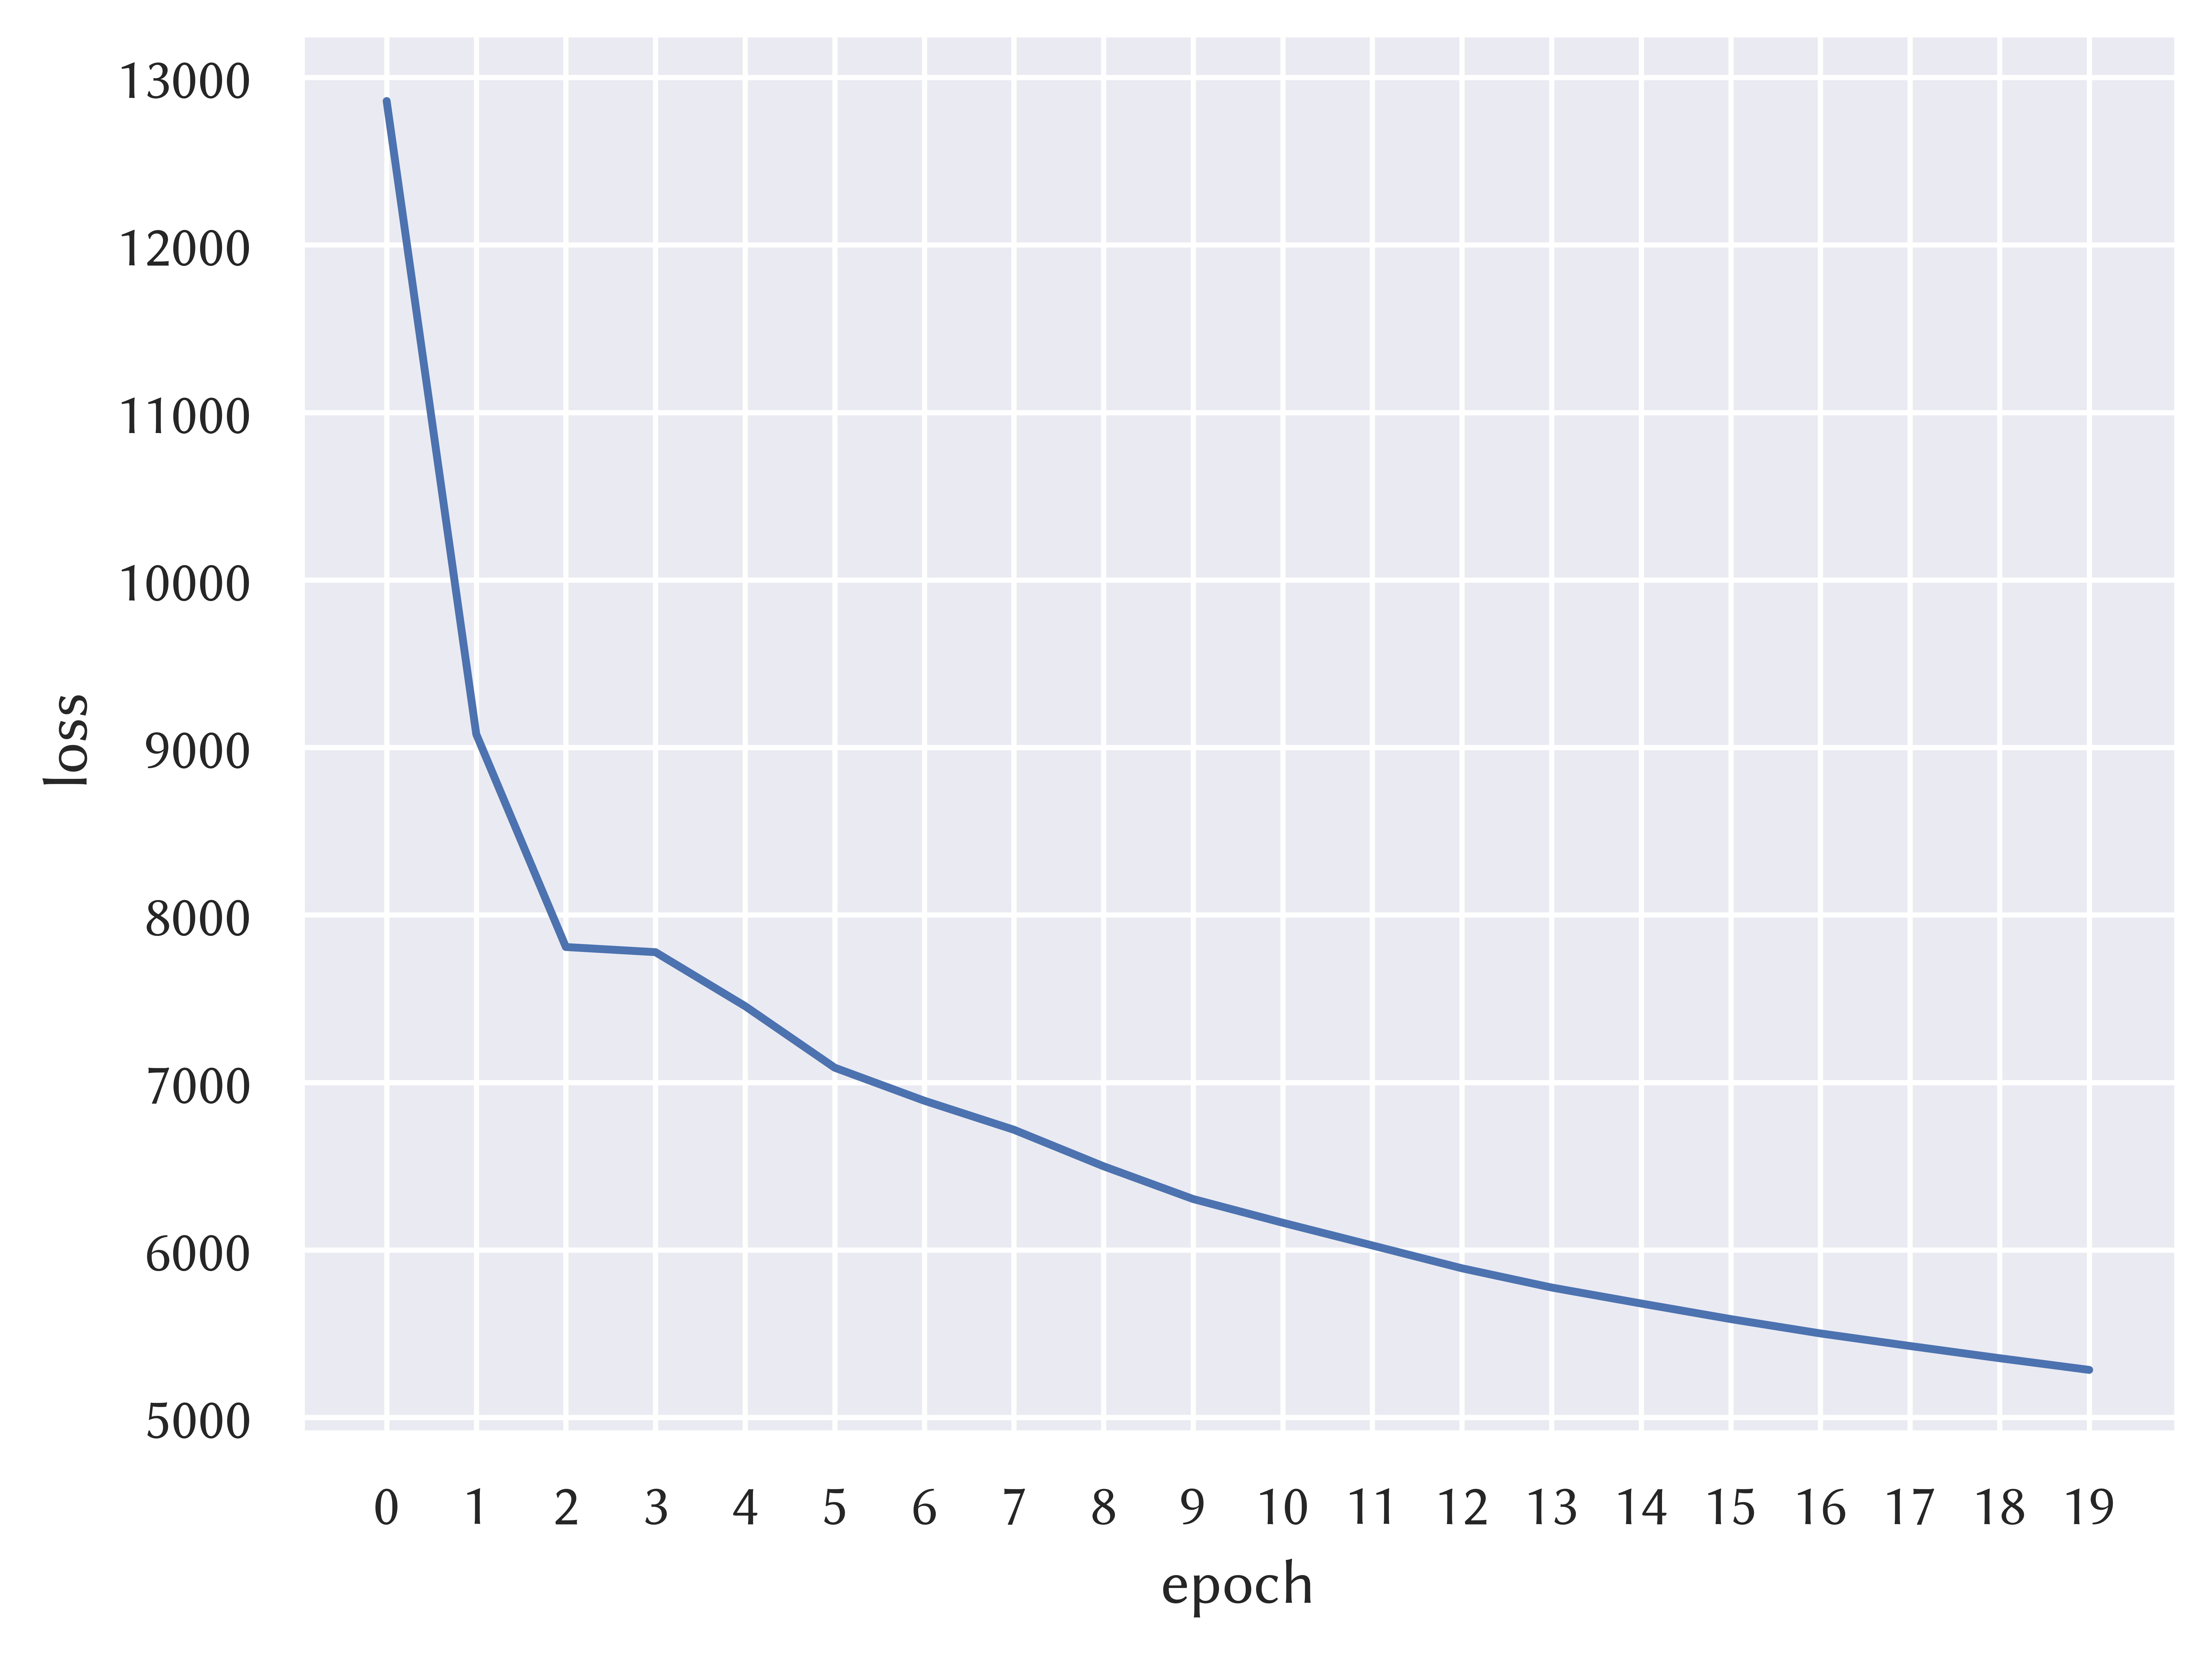
\includegraphics[width=0.7\textwidth]{fig/log.png}    
\end{center}
\end{frame}

\begin{frame}{Segment-based model}
    \begin{figure}[h]
        \centering
        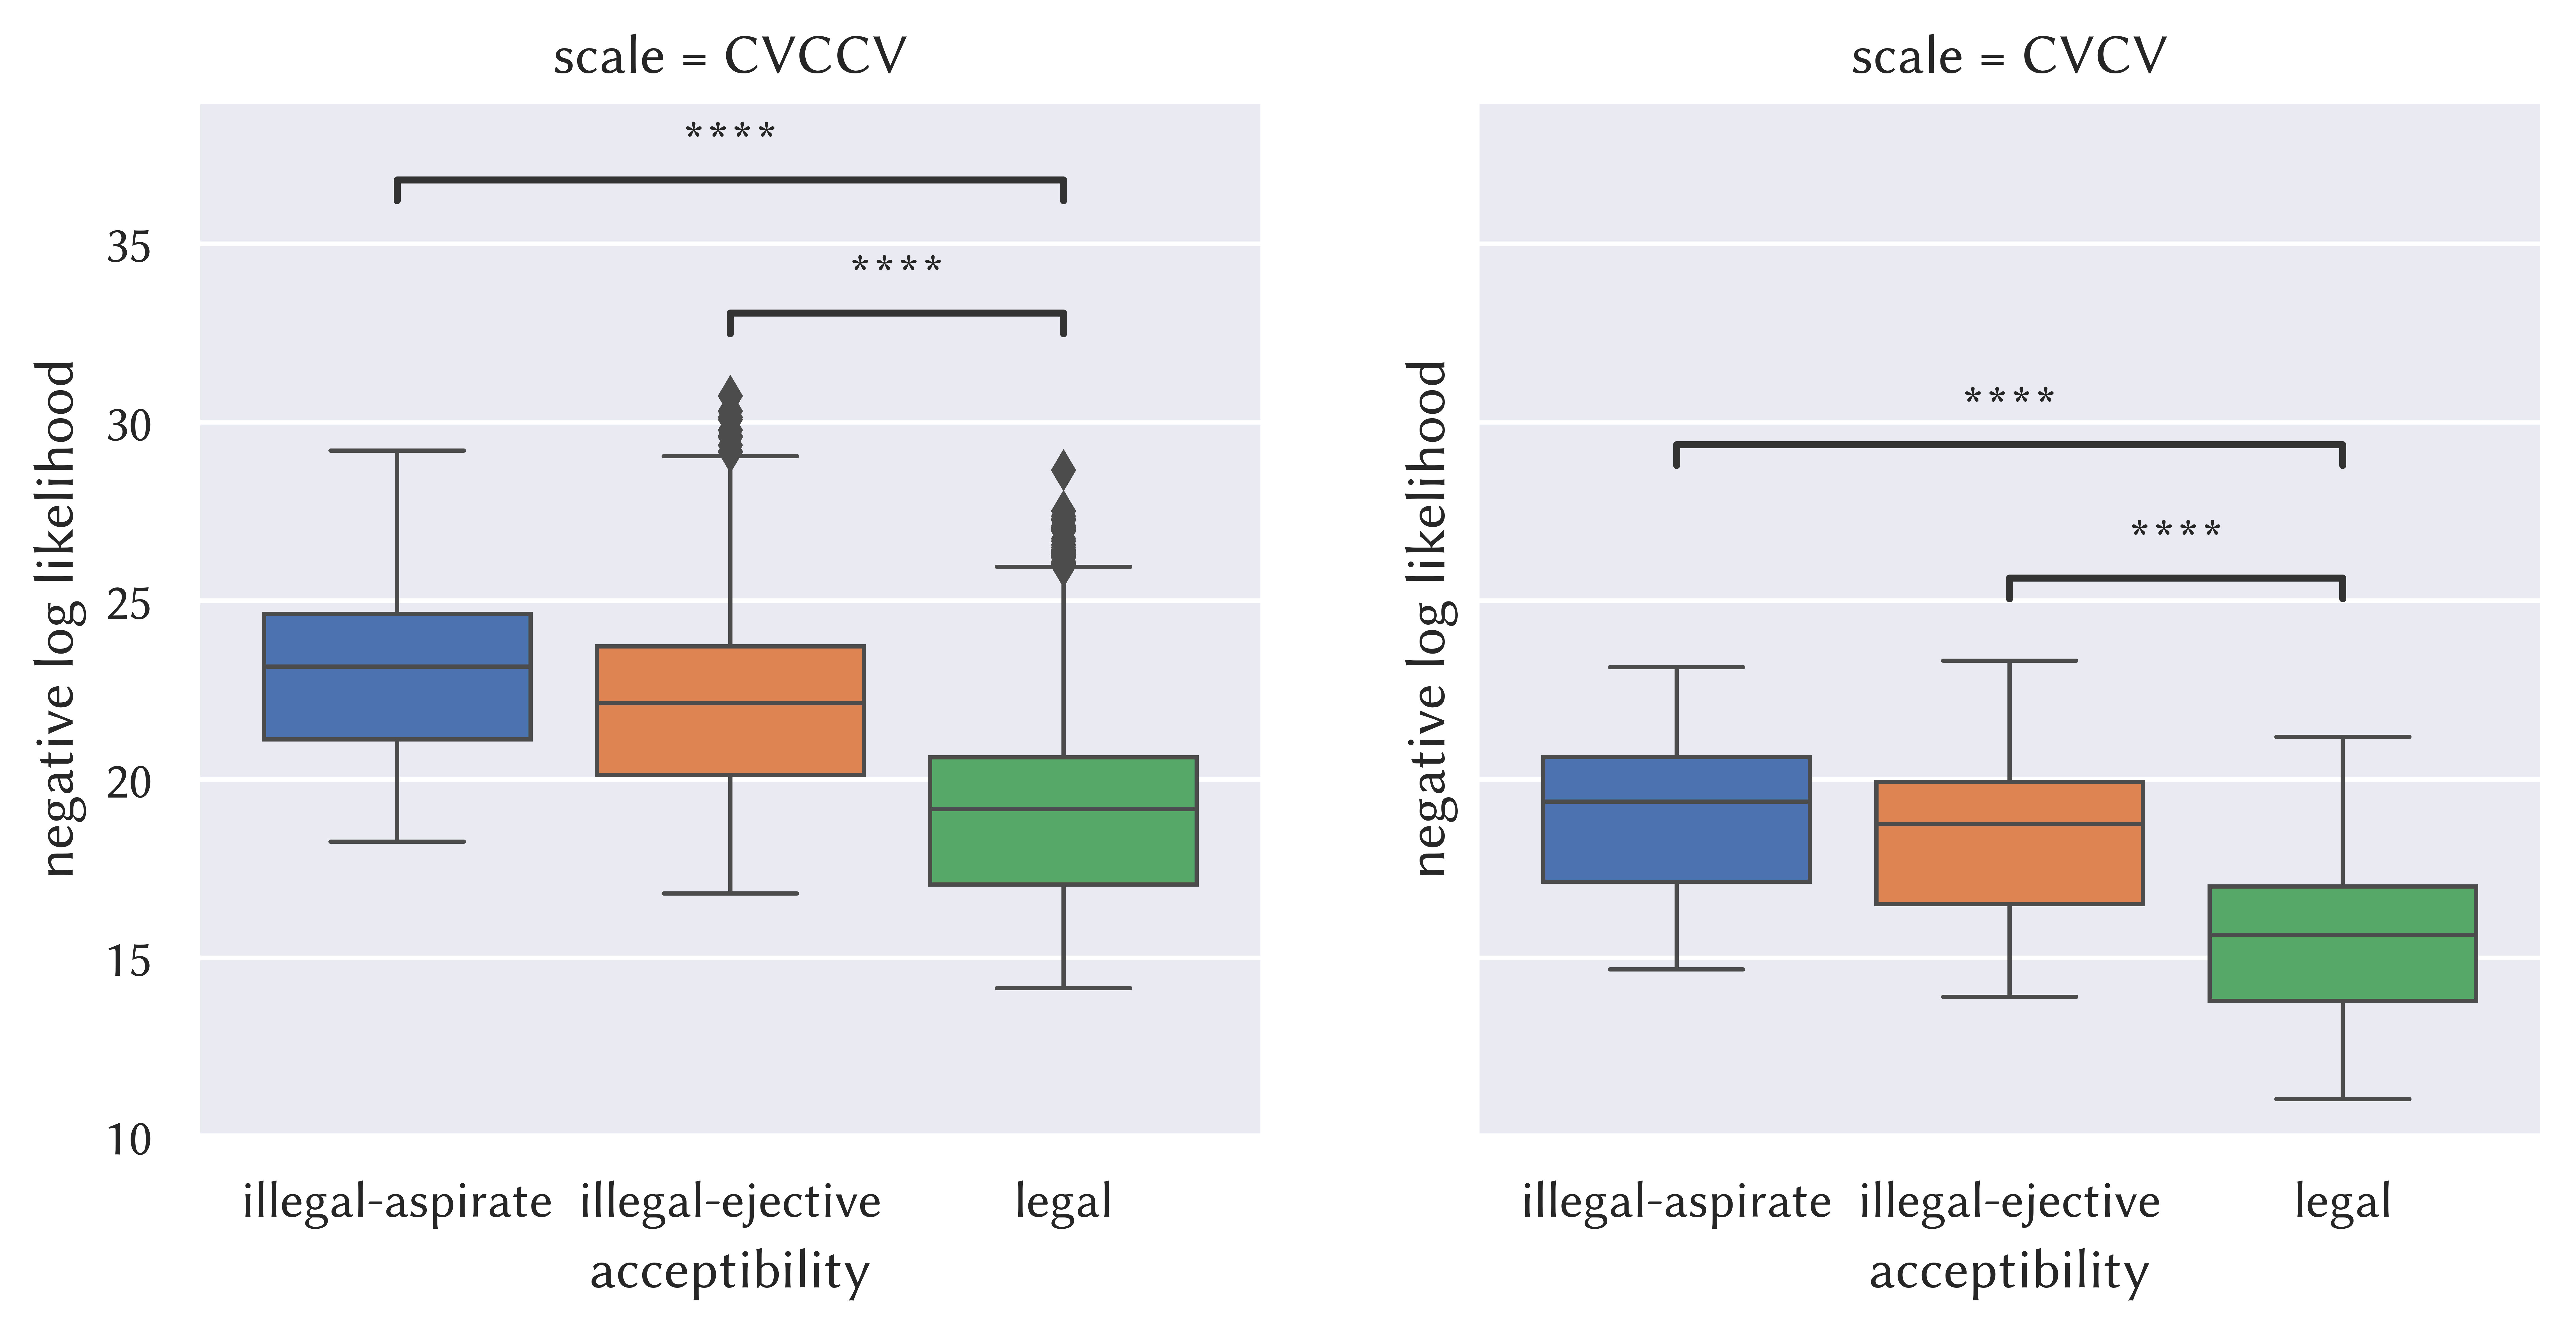
\includegraphics[width=\textwidth]{fig/fig:boxplot-seg.png}
    \end{figure}
\end{frame}

\begin{frame}{Feature-based model}
    \begin{figure}[h]
        \centering
        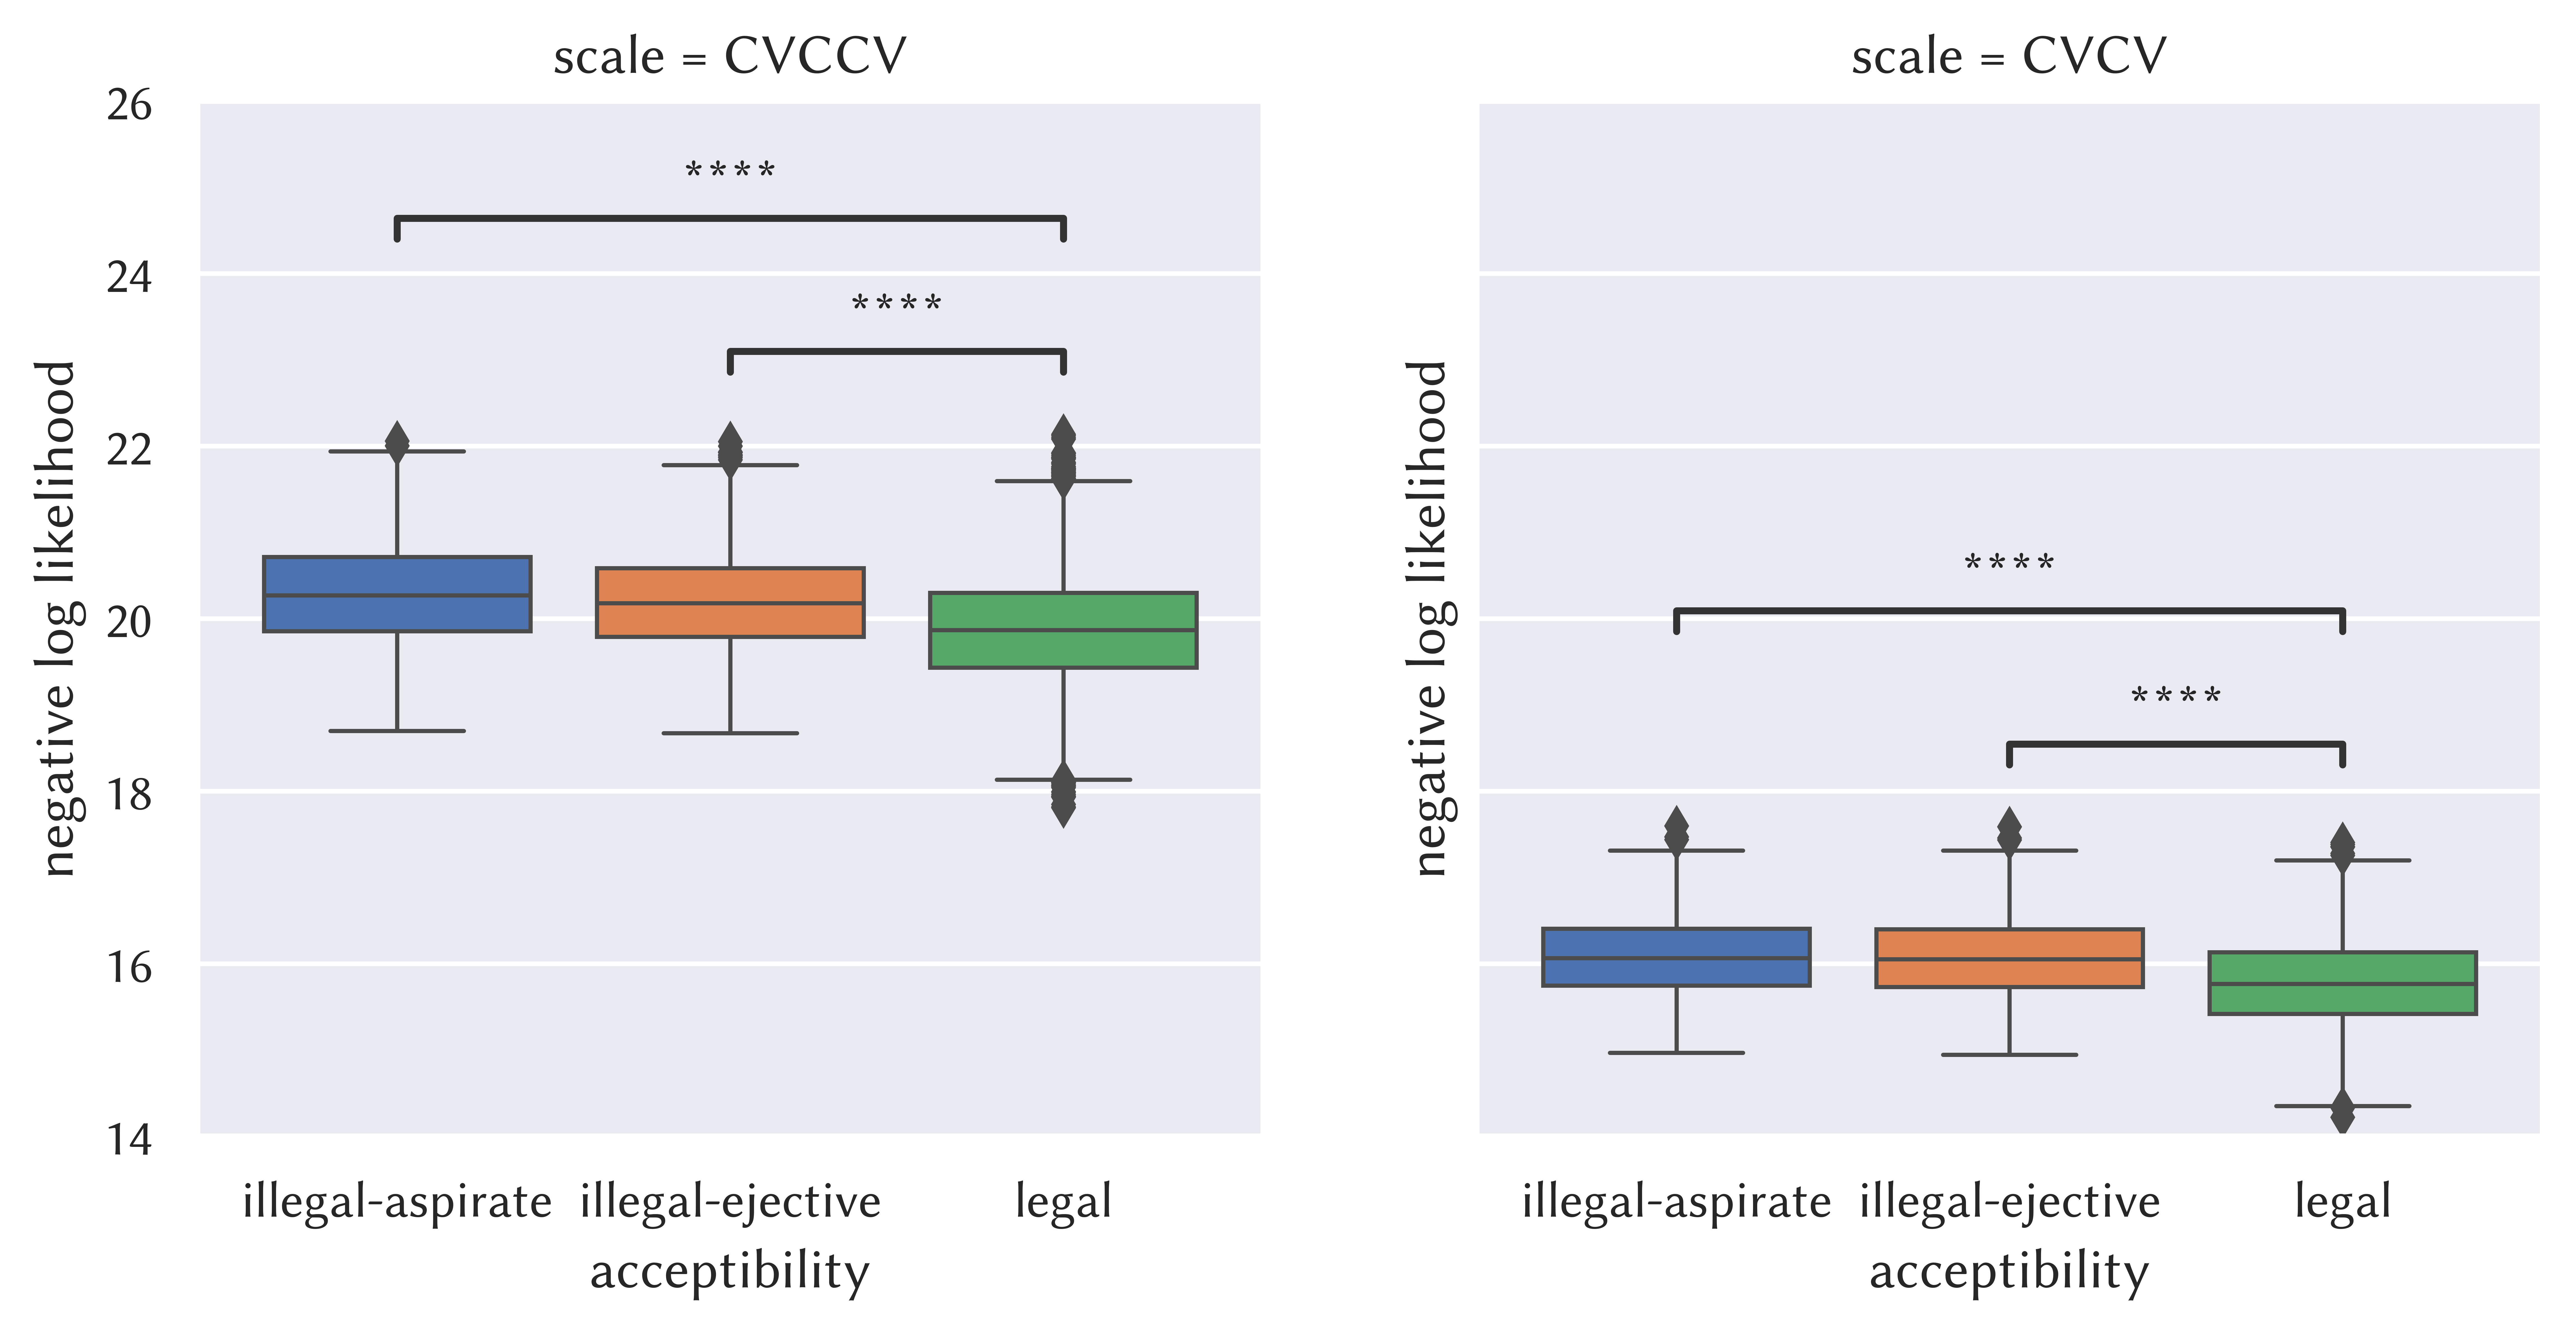
\includegraphics[width=\textwidth]{fig/fig:plot-feat-box.png}
    \end{figure}
\end{frame}




\begin{frame}{Conclusion}
    \begin{itemize}
    \item SP phonotactic model is capable of generalizing nonlocal phonotactics at arbitrary distance.
    \item SP phonotactics learner correctly distinguishes the acceptability of Quechua nonce words.

    \end{itemize}
    
\end{frame}

\begin{frame}{Acknowledgement}
 I thank Jeff Heinz, Adam Jardine, Bruce Tesar, Adam McCollum for their comments and insights. My special thanks are extended to Brian Pinsky, Liam Schramm, and Yu Cao for providing the valuable suggestions on the implemented Python code.

\vspace{0.5cm}
\begin{figure}[h]
    \centering
\resizebox{0.5\textwidth}{!}{
    
\includegraphics{fig/rutgers-logo.png}}
\end{figure}
\end{frame}

\appendix

\begin{frame}{Blocking effect}
    
\end{frame}
        

\begin{frame}{Forward algorithm}
\centering
\resizebox{\textwidth}{!}{
\begin{algorithm}[H]
% \SetAlgoLined
 \textsf{nll} $\leftarrow 0$\;
 \For{word in $S$}{
 state $\leftarrow$ 0 in each automaton $\mathcal{M_{\textit{j}}}$\;
\For{$\sigma_i$ in word}{
Initialize a lookup dictionary $D$ for $\prod_{j=1}^{K}T(\mathcal{M}_{j}, q, \sigma^{\prime})$\;
\For{$\mathcal{M_{\textit{j}}}$ in automata}{
\For{$\sigma^{\prime}$ in alphabet}{
Update the lookup dictionary with $\sigma^{\prime}$\;
}
Update the state on $\mathcal{M_{\textit{j}}}$\;
}  
\textsf{nll} $\leftarrow$ \textsf{nll} - log(\textsf{Coemit}(\textit{$\sigma_i$}))
}
}
\KwResult{Negative log likelihood \textsf{nll} of $S$}
% \caption{Forward algorithm}
\end{algorithm}
}
\end{frame}
\section{Reference}

\setbeamertemplate{background}{\begin{tikzpicture}
		% set up the entire slide as the canvas
		\useasboundingbox (0,0) rectangle(\the\paperwidth,\the\paperheight);
		% the background
		\fill[color=white] (0,0) rectangle(\the\paperwidth,\the\paperheight);
		\end{tikzpicture}
	 }
\begin{frame}[allowframebreaks,fragile]{}
\renewcommand*{\bibfont}{\small}
  \bibliography{refs}
  \bibliographystyle{apacite}
% \printbibliography[title = Selected references]
\end{frame}

